\documentclass[final,hyperref={pdfpagelabels=false}]{beamer}
\usepackage{grffile}
\mode<presentation>{\usetheme{PosterLogProb}}
%\mode<presentation>{\usetheme{I6pd2}}
\usepackage[english]{babel}
\usepackage[latin1]{inputenc}
\usepackage{amsmath,amsthm, amssymb, latexsym}
\usepackage{epsfig}

%\usepackage{algorithm}
%\usepackage{algorithmic}

%\usepackage{times}\usefonttheme{professionalfonts}  % obsolete
%\usefonttheme[onlymath]{serif}
%\boldmath
\usepackage[orientation=portrait,size=a0,scale=1.4,debug]{beamerposter}
% change list indention level
% \setdefaultleftmargin{3em}{}{}{}{}{}
\providecommand\thispdfpagelabel[1]{}
\setbeamertemplate{bibliography entry title}{\color{black}}
\setbeamertemplate{bibliography entry location}{}
\setbeamertemplate{bibliography entry note}{}


%\usepackage{snapshot} % will write a .dep file with all dependencies, allows for easy bundling

\usepackage{array,booktabs,tabularx}
\newcolumntype{Z}{>{\centering\arraybackslash}X} % centered tabularx columns
\newcommand{\pphantom}{\textcolor{ta3aluminium}} % phantom introduces a vertical space in p formatted table columns??!!

\listfiles

\usepackage{amsthm}
%%%%%%%%%%%%%%%%%%%%%%%%%%%%%%%%%%%%%%%%%%%%%%%%%%%%%%%%%%%%%%%%%%%%%%%%%%%%%%%%%%%%%%


 \title{\huge\bfseries\hspace*{-1em} Aplica��o de Pr�ticas de Usabilidade no processo de desenvolvimento emp�rico de software.}
\date{}
\author{\large J�natas Medeiros
\and Rodrigo Medeiros
\and Paulo Meirelles 
}
\institute[UnB]{LAPPIS -- Universidade de Bras�lia, Brasil}

%%%%%%%%%%%%%%%%%%%%%%%%%%%%%%%%%%%%%%%%%%%%%%%%%%%%%%%%%%%%%%%%%%%%%%%%%%%%%%%%%%%%%%
\newlength{\columnheight}
\setlength{\columnheight}{105cm}


%%%%%%%%%%%%%%%%%%%%%%%%%%%%%%%%%%%%%%%%%%%%%%%%%%%%%%%%%%%%%%%%%%%%%%%%%%%%%%%%%%%%%%
\begin{document}
\begin{frame}
  \begin{columns}
    % ---------------------------------------------------------%
    % Set up a column 
    \begin{column}{.49\textwidth}
      \begin{beamercolorbox}[center,wd=\textwidth]{postercolumn}
        \begin{minipage}[T]{.95\textwidth}  % tweaks the width, makes a new \textwidth
          \parbox[t][\columnheight]{\textwidth}{ % must be some better way to set the the height, width and textwidth simultaneously
            % Since all columns are the same length, it is all nice and tidy.  You have to get the height empirically
            % ---------------------------------------------------------%
            % fill each column with content
%\vfill
\begin{block}{What is Kalibro}
  \begin{itemize}

	\item Kalibro Metrics goal is to improve the readability of source code metrics. It
	allows a source code metric user to create a configuration of thresholds
	associated with qualitative evaluation, including comments and recommendations.

	\item Using these configurations, Kalibro provides that a ``view layer'' shows metric results in a friendly way,
	helping software engineers to spot design flaws to refactor, project managers
	to control source code quality, and software adopters and researchers to compare
	specific source code characteristics across free software projects.

	\item These configurations are shared among its users via the Kalibro Web Service and
	a source code tracking network to enhance metric results interpretation.
        
  \end{itemize}              
\end{block}

%-------------------------------------------------------------------------------
\vfill
\begin{block}{Why Kalibro?}
	\begin{itemize}
		\item We have identified, in particular, two limitations from current available tools,
		i.e., lack of the following features:

		\begin{itemize}

		\item To collect automatically source code metrics values independent of the
		programming language;  
		\item To interpret measurement results, associating them with source code
		quality.
	
		\end{itemize}
		
	\end{itemize}

\end{block}


%-------------------------------------------------------------------------------
\vfill
\begin{block}{Kalibro Features}
	\begin{itemize}

		\item Download source code from Subversion, Git, Mercurial, Baazar, and CVS repositories.

		\item Download source code from local and remote zip and tarball (.tar,
		.tar.gz, and tar.bz) files.

		\item Creation of configurations, i.e., a set of metrics for being used in the
		evaluation of a software source code.
		
		\item Creation of ranges associated with a metric and a qualitative evaluation.

		\item Creation of new metrics (via JavaScript) based on the ones provided by
		the metric collector tool.

		\item Calculation of statistics results for higher granularity modules
		(e.g. average LOC of classes inside a package).

		\item Possibility of exporting results to a CSV (comma-separated values) file.

		\item Calculation of a grade for the source code analysis projects, based on
		given weights for each metric and grades for ranges. This allows cross-project
		comparisons.

		\item Possibility of making interpretation more user-friendly by associating
		colors with ranges.

	\begin{figure}
	  \begin{center}
	    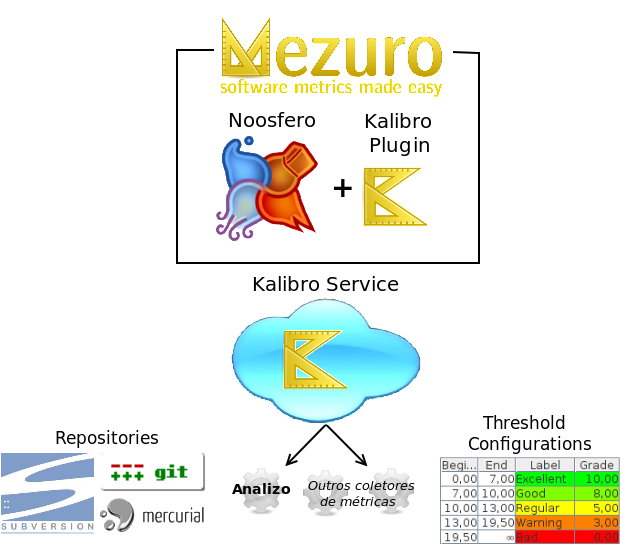
\includegraphics[scale=1.5]{figures/interactions.png}
	    \caption{kalibro interation diagram.}
	    \label{fig:background:free-software-repository}
	  \end{center}
	\end{figure}

	\end{itemize}
\end{block}

\vfill
        

}
\end{minipage}
\end{beamercolorbox}
\end{column}
% ---------------------------------------------------------%
% end the column

% ---------------------------------------------------------%
% Set up a column 
\begin{column}{.49\textwidth}
  \begin{beamercolorbox}[center,wd=\textwidth]{postercolumn}
    \begin{minipage}[T]{.95\textwidth} % tweaks the width, makes a new \textwidth
      \parbox[t][\columnheight]{\textwidth}{ % must be some better way to set the the height, width and textwidth simultaneously
        % Since all columns are the same length, it is all nice and tidy.  You have to get the height empirically
        % ---------------------------------------------------------%
        % fill each column with content

        \begin{block}{Kalibro Architecture}

	\begin{itemize}
          	\item \textbf{KalibroCore} is the heart of Kalibro Metrics. It contains
		all logic, including database access, metric collector tool interaction,
		statistics computation and compound metric scripts evaluation. It includes a
		Java abstract class (KalibroFacade) to access all its functionality.

		\item \textbf{KalibroService} is a Web Service interface for using Kalibro.

        \end{itemize}
          	
        \end{block}
             
	\vfill
\begin{block}{Kalibro Plug-in for Mezuro networking}
          \begin{itemize}

		\item A social network to track source code metrics.

		\begin{itemize}

			\item This environment promotes
			an open and collaborative networking to analyze hundreds of thousands
			software projects, specially Free Software, through an automated tracking
			of their source code repositories.
		\end{itemize}


		\item Mezuro is a powerful environment to enhance Kalibro features,
		using the social network potential.
		
		\begin{itemize}
			\item The idea is based on the fact that people improve their writing skills when they
			read good books and papers. Similarly, software engineers can increase the
			quality of their source codes reviewing good and clean codes.

			\item a developer can find through source code metrics software projects implemented in the same context 				and language, they can compare their source code characteristics and know other related projects.
	          \end{itemize}

		\item Users just need to give a source code repository URL.

		\item Users can access the source code analysis report
		from an asynchronous way, i.e. when they wish or need.

		\item The history of source code metric values and analysis are recorded.  

		\item All free and public project analysis are available to any user.

		\item Any user can suggest metric threshold configurations and share them
		on the Mezuro network.

          \end{itemize}
        \end{block}
\vfill
      }
      % ---------------------------------------------------------%
      % end the column
        \end{minipage}
      \end{beamercolorbox}
    \end{column}
    % ---------------------------------------------------------%
    % end the column
  \end{columns}
  %\vskip1ex
  % \tiny\hfill\textcolor{ta2gray}{Created with \LaTeX \texttt{beamerposter}  \url{http://www-i6.informatik.rwth-aachen.de/~dreuw/latexbeamerposter.php}}
  
\end{frame}
\end{document}


%%%%%%%%%%%%%%%%%%%%%%%%%%%%%%%%%%%%%%%%%%%%%%%%%%%%%%%%%%%%%%%%%%%%%%%%%%%%%%%%%%%%%%%%%%%%%%%%%%%%
%%% Local Variables: 
%%% mode: latex
%%% TeX-PDF-mode: t
%%% End:

% LocalWords:  ABox ABoxes PSAT
